\section{Operations Management}
\label{sec:ops}
\subsection{Alignment of Business and Operational Strategies}
\label{sec:ops1}
Future feeders is a meal delivery service intending to offer school lunches with less effort and more convenience. The product offers a fresh, filling and healthy lunchbox meal delivered directly to partnering schools. Future feeders is an app based school lunch delivery service. It aims to partner with schools, offer convenience to parents, and delight children. The draw card being on the quality consistency of our product.

Future Feeders will adopt a lean business strategy. To complement this, operations will adopt a just-in-time  supply strategy. The principle that underpins just-in-time strategy is that supply inventory should be ``pulled'' on request to satisfy demand. Future Feeders will make use of both pull and push systems to leverage the advantages of both systems. A pre-order system will determine demand two days prior to delivery. Stock procurement is subsequently managed, thereby eliminating waste by reducing the amount of inventory and the cost of storing the goods. This will also aid in keeping the cost price of stock variable. Orders are pre-planned to ensure that the correct amount of stock is available for the specific days and the right amount of quantity is prepared each day. This characteristic is conveyed in Figure~\ref{fig:transform}.

\begin{figure}[h]
    \centering
    \captionsetup{justification=centering,margin=2cm}
    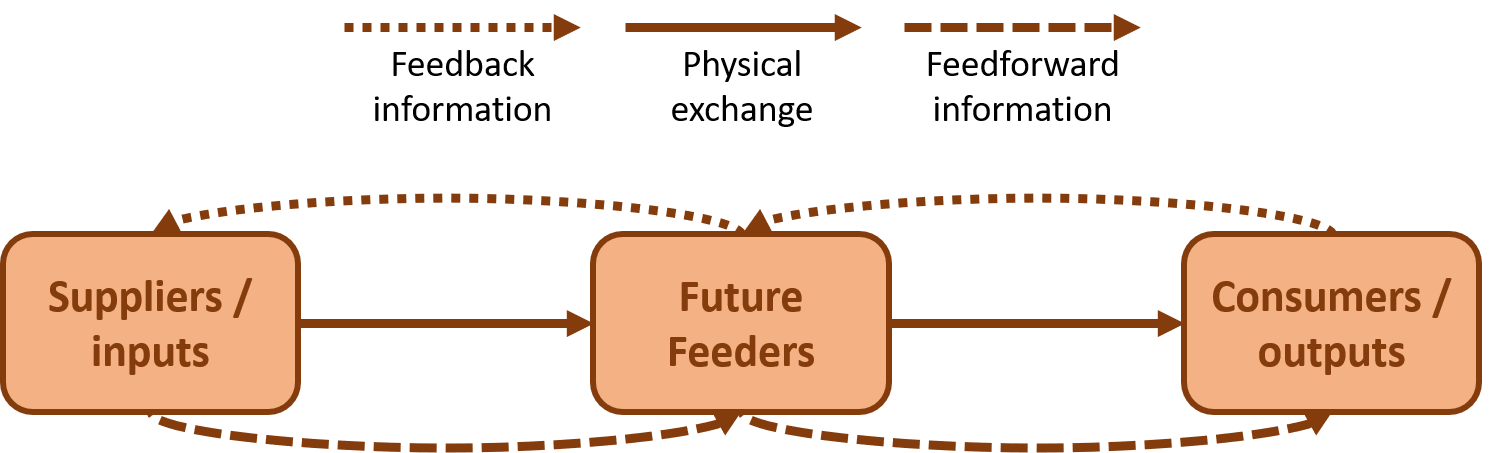
\includegraphics[width=\textwidth]{op_transform.png}
    \caption{Push and pull operation control \protect\cite{ops_book}.}
    \label{fig:transform}
\end{figure}

The distribution process would be pushed through because the daily demand is known through pre-ordering. The meals would be prepared, packed, and distributed each day. The reason for opting for a just-in-time strategy is that the meals will vary from day to day, meals would be prepared in terms of season (having lighter meals during the summer months and having heavy/warm meals during the winter season) taking into consideration the holiday breaks that schools have as well, making the business subject to seasonal variations in demand.

Quality control is a crucial factor that would have to be continuously managed. This must extend to sourcing the raw materials (input process), making the food (transformation process) and finally distributing it to the children (output process). Future Feeders has a challenging task when outsourcing its products because we would have to consider the quality standards from different suppliers and supply network design. The supply and customer network is included as Figure~\ref{fig:spider} in Appendix~\ref{app:network}.

\begin{itemize}
    \item \textbf{Multi-sourcing} would influence the quality standard required although this would help with keeping. The benefit of multi-sourcing would be a reduction in costs and offering redundancy \cite[p. 337]{ops_book}.
    \item \textbf{Single sourcing} would ensure that consistency and supplier control is better managed. The potential downside is the single supplier dependency \cite[p. 337]{ops_book}.
\end{itemize}

Future Feeders would look to single-source perishable goods and multi-source the non-perishable goods. Procurement would be done on a just-in-time basis because of the level of quality required. Additionally, product freshness and quantity demanded can be managed.

Future Feeders core function is to produce the food for the lunch boxes. Distribution should be outsourced in an effort to restructure fixed costs to variable costs and benefit from economies of scale. To ensure that the quality of standard is adhered to, Future Feeders would have employees waiting at the different schools to accept delivery. This is to ensure that the food delivered can still be given out to the students. Quality and assurance must be managed at a face-to-face level i.e. Future Feeders must distribute the individual lunches at the school.


\subsection{Process Design}
\label{sec:ops2}
As a business that is concerned with producing food, the general process classification would fall into that of a batch process \cite[pp. 74-96]{ops_book}. Batch processes can exhibit a wide range of volume and variety characteristics. Future Feeders intends to maintain a high quality output but it is imperative that throughput can also be managed.

There is some overlap in batch processes with jobbing and mass processes. Future Feeders will require a large output volume to remain financially viable. Large volume output will put a strain on variety. Although day-to-day variation will occur, on the day variations in terms of daily menu offering must be limited. The high volume work will by necessity require an assembly line characteristic process. This means that Future Feeders will tend toward a continuous process flow, with repeated or divided tasks. Dividing the process into sub-processes will allow high volumes to be achieved. By implication, within the batch processing characteristic, Future Feeders will tend toward the mass process region as shown in Figure~\ref{fig:op_design}.

\begin{figure}[H]
    \centering
    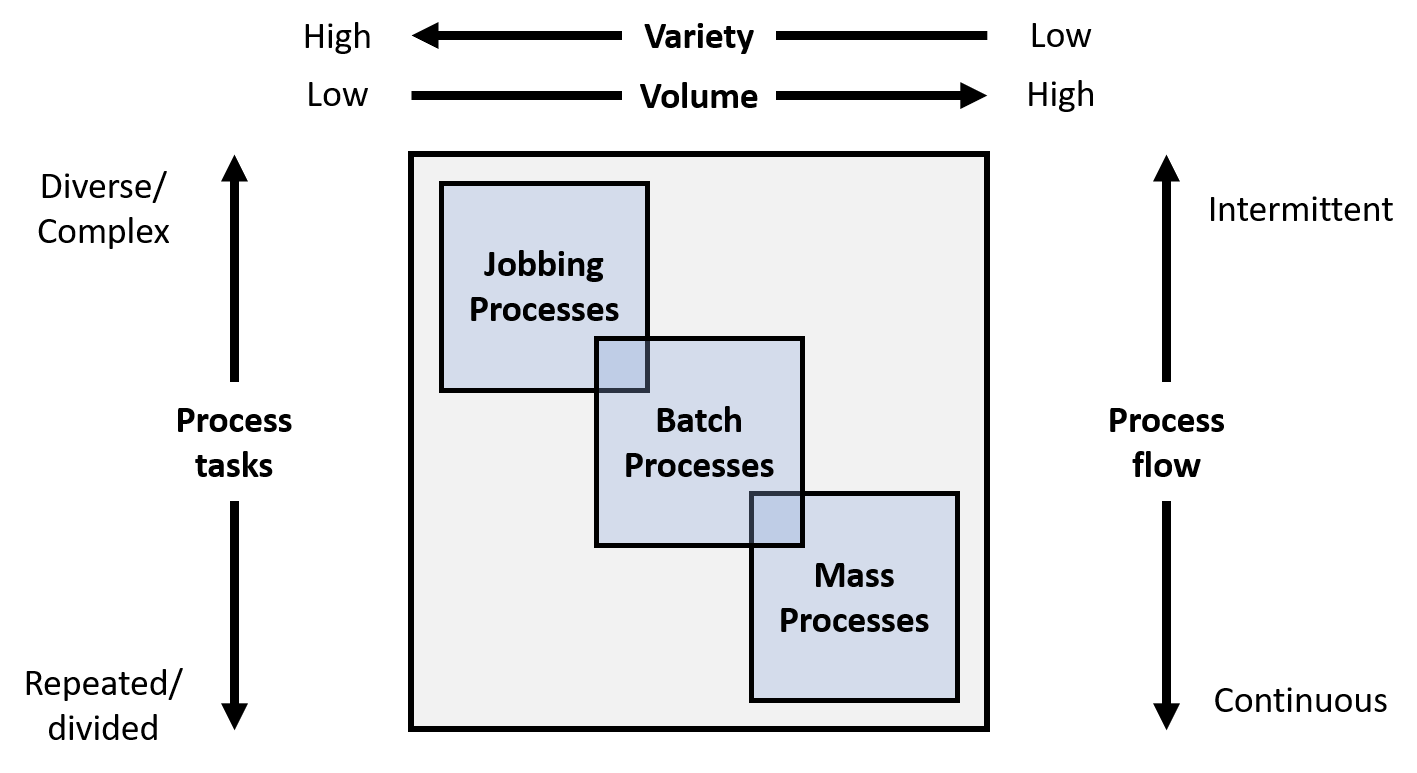
\includegraphics[width=0.9\textwidth]{op_design.png}
    \caption{Future Feeders process type classification (modified from \protect\citeauthor{ops_book}, \protect\citeyear{ops_book}, p. 80.)}
    \label{fig:op_design}
\end{figure}

It is important to realise that Future Feeders intends to offer convenience to its customers and timing is imperative when delivering lunches to children. Taking too long to produce or package lunches may cause a delay in delivery. Similarly, if the distribution company is late for collection, the same problem occurs.

With the above in mind, Future Feeders will require intimate knowledge of the daily operation schedule. With the daily output known, required materials must be requisitioned in a pull order. This is in order to maintain freshness. This will be discussed in Section~\ref{sec:ops3}. The overriding process design or value chain is included in Appendix~\ref{app:process} as Figure~\ref{fig:op_process}.

\subsection{Scheduling and Managing Work In Progress (WIP)}
Future Feeders will not be able to realise high gross, operating, and earnings before tax margins unless the operations procedure is strategically managed. Future Feeders runs a very time sensitive operation. Allocating time adequately, efficient use of resources, and scheduling is critically important. The following operational factors are incorporated into Future Feeders operational procedures:

\begin{itemize}
    \item \textbf{Push demand} - subscription services with a two day allow quantity demanded to be ascertained. On the day of delivery. Output is pushed to meet demand for each day.
    \item \textbf{Pull supply} - based on known quantity demanded, supply of raw material can be arranged and met.
    \item \textbf{Upfront scheduling} - with quantity demanded known and materials required organised, scheduling can occur. This includes time and employee scheduling to meet demand on time.
\end{itemize}

To illustrate this, Appendix~\ref{app:schedule} includes a menu (Table~\ref{tab:menu}) that the customer sees. In this instance, 120 lunches are ordered. With the menu known, tasks can be defined for the day delivery must be met, shown in Table~\ref{tab:split}. If delivery must occur at 10:30 and twenty minutes are required, the lunches must be ready by 10:05 at the latest. Factoring into this is the freshness requirement. This means that certain components may not be ready before they are required. This is aligned with a JIT system. Scheduling is made upfront, this is shown by the Gantt chart in Figure~\ref{fig:gantt}. This allows Future Feeders to contact shot-time staff as required to mitigate process strain. If the kitchen can handle 200 deliveries by design, and effective capacity with, staffing considerations, is 150, process utilisation and efficiency, in this instance, are shown in Equation~\ref{eq:uti} and Equation~\ref{eq:eff} respectively:


\begin{equation}
\text{Utilisation} = \frac{120}{200} = 60~\%
\label{eq:uti}
\end{equation}

\begin{equation}
\text{Efficiency} = \frac{120}{150} = 80~\%    
\label{eq:eff}
\end{equation}

The effect of the operation is in an attempt to reduce waste and increase operational effectiveness. Planning each day can identify process bottlenecks, lead times required, where slack can be introduced, and where staff can be better utilised.

Evidently, day-to-day menu variations will change. A high variability in demand is subsequently expected, which is also subjected to seasonal demand. By implication variety will be low. This will also impact on the volume. Quality assurance being of critical importance means that visibility will be by relatively high by necessity. This is qualitatively included in Appendix~\ref{app:4v} as Figure~\ref{fig:4v}. The combination of volume, variety, variation, and visibility is related to McDonald's operating procedures highlighted by \citeauthor{mcdonalds}, \citeyear{mcdonalds}, (pp. 672-701).

\label{sec:ops3}
